\section{Shortcomings of Application Parallelism} \label{sec:darksilicon}

Dreslinski et al.~\cite{dreslinski2010near} state ``More gates can now fit on a
die, but a growing fraction cannot actually be used due to strict power
limits.'' This issue is commonly referred to as dark silicon.  While the number
of transistors on a given die has been doubling every generation, the number of
transistors that can be powered for a fixed power budget has not been increasing
due to the slowing of transistor energy scaling. Since power budgets have not
been increasing past the limits defined by air cooling, a situation has arisen
where future generations of chips will potentially have more transistors than
can be powered at any given time.  Several recent
works~\cite{Esmaeilzadeh2011Dark-silicon-an,Hardavellas:2011de} have looked at
the impact of dark silicon on computing in the near future. 

Dark silicon seemingly presents an opportunity for near-threshold computing, and
as a way of addressing the large area overheads of the clustering architectures
discussed in Section~\ref{sec:clustering}. By reducing the power consumed
per-core, more cores can be simultaneously powered. Since these cores could not
be powered in a super-threshold chip, this represents an opportunity for
near-threshold chips to regain performance compared to super-threshold
operation.

\begin{figure}[thpb] \centering
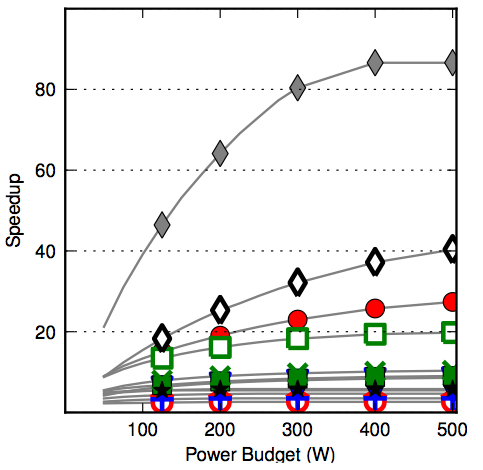
\includegraphics[width=0.3\textwidth]{esmaeilzadeh_power_speedups.png}
\caption{Projected speedups on PARSEC benchmarks while the chip power limit (and
therefore the number of cores) is
increased.~\cite{Esmaeilzadeh2011Dark-silicon-an}} \label{fig:power_speedups}
\end{figure}

While dark silicon is an opportunity for devices to reach higher levels of
integration, recent studies analyzing dark silicon have not born out the
promise of higher levels of performance with increasing core counts.  Work by
Esmaeilzadeh et. al~\cite{Esmaeilzadeh2011Dark-silicon-an} developed an
analytical model analyzing the impact of dark silicon for a range of CMP
configurations in future process technologies. They show projected speedups for
these configurations using the PARSEC benchmark suite, which represents
workloads similar to the SPLASH2 benchmark suite used in the previously
discussed clustering architecture papers~\cite{dreslinski2010near,Zhai:2007kn},
indicating that both works are targeting similar applications. This analytical
model does project that dark silicon will become a significant portion of CPU
area in the near future, dominating as soon as 2016 with a conservative scaling
model. However, the authors also analyze the case where the power constraint is
lifted, which allows more cores to be powered and reduces the amount of dark
silicon. Figure~\ref{fig:power_speedups} shows the projected speedups on
different PARSEC benchmarks as the chip power is increased. The paper projects
that if the amount of parallelism in applications were increased to 99\%, then
the best case speedup for power limited cores in \SI{8}{\nano\meter} is 15x
relative to a quad-core Nehalem processor at \SI{45}{\nano\meter}. However, as
shown in Figure~\ref{fig:power_speedups}, with an unconstrained power budget,
and the same current amount of application level parallelism, 8 out of 12
PARSEC benchmarks achieve no more than 10x speedup.  What this indicates is
that the amount of parallelism in general-purpose parallel workloads is
currently not exploitable even by future power constrained multi-core chips.
While near-threshold computing would allow more chips to be powered, it would
not realize a significant speedup on most general-purpose parallel workloads
due to the lack of exploitable parallelism.

\begin{figure}[thpb] \centering
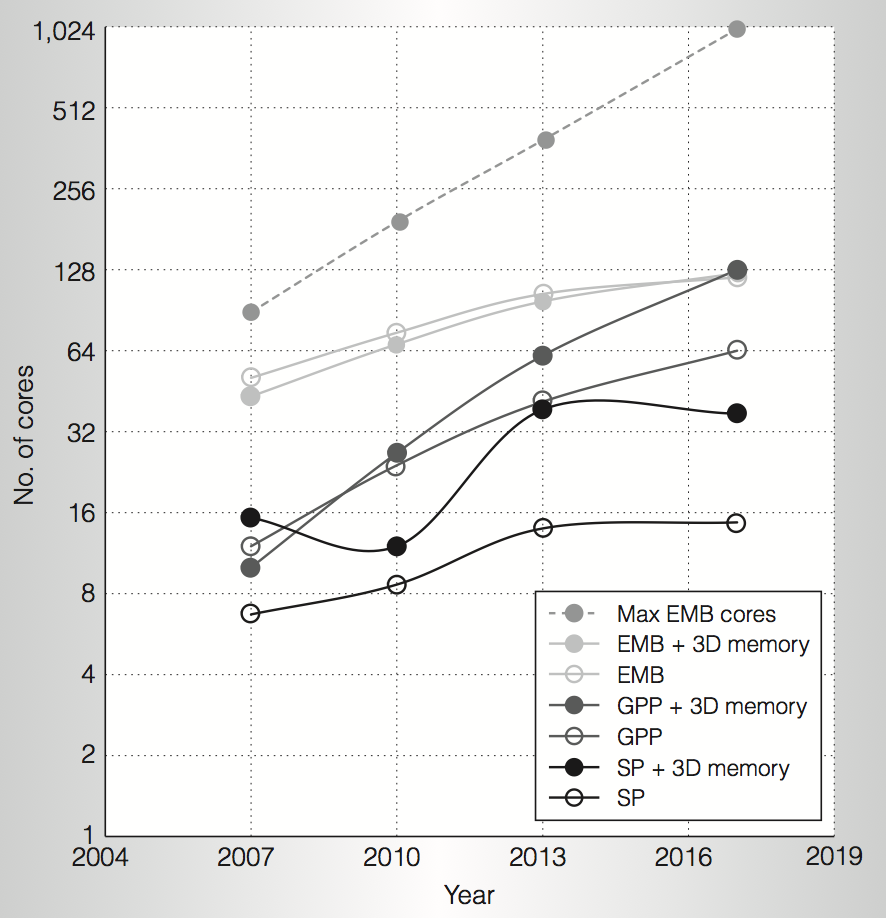
\includegraphics[width=0.4\textwidth]{hardavellas_core_counts.png}
\caption{Projections for core count scaling.~\cite{Hardavellas:2011de}}
\label{fig:core_counts} \end{figure}

\begin{figure}[thpb] \centering
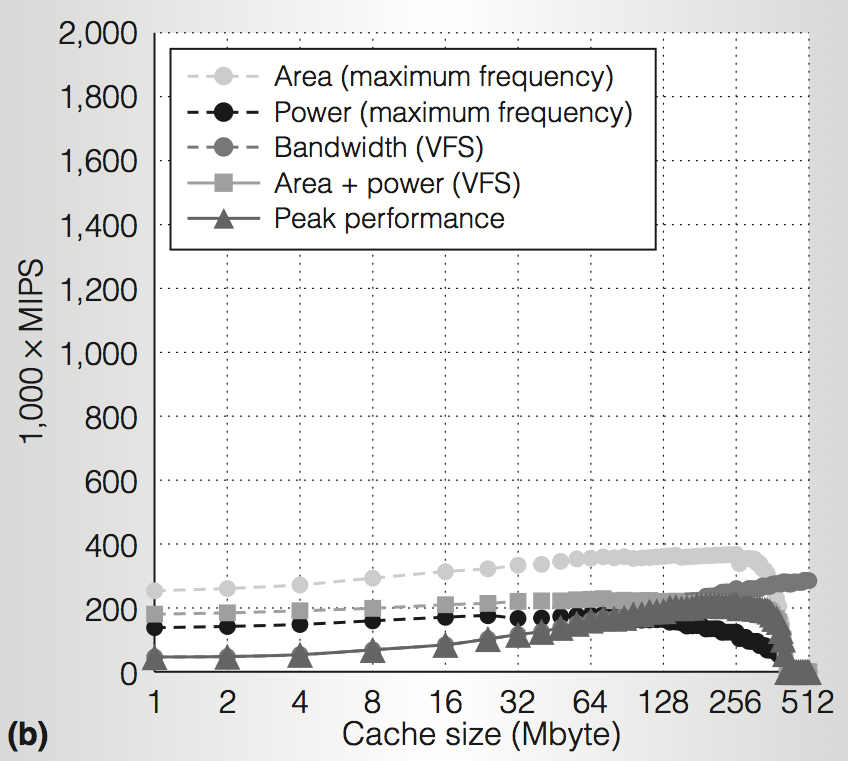
\includegraphics[width=0.4\textwidth]{hardavellas_emb_performance.png}
\caption{Embedded core scaling.~\cite{Hardavellas:2011de}}
\label{fig:emb_performance} \end{figure}

Further work by Hardavellas et al.~\cite{Hardavellas:2011de} confirms the
observation that future speedups are limited by application level parallelism,
not power constraints. In this study the authors built an analytical chip performance model for
different types of cores, including low-power embedded cores (EMBs) similar to
an ARM11 MPCore, and modeled how the performance of these chips scale in future
process technologies given area,
power, and memory bandwidth constraints. Figure~\ref{fig:core_counts} shows
projected core count scaling trends in future process technologies. The
difference between the ``Max EMB cores'' line and the ``EMB'' line represents
the difference in how many cores can fit on a die versus how many can be powered
given current power constraints.  Their model projects that in 2017 over 1024
cores will be able to fit on a die, but only 12\% of them will be able to be
powered at any given time.  Again, this looks like an opportunity for
near-threshold computing to increase core counts over traditional
super-threshold CMPs.

Figure~\ref{fig:emb_performance} shows the maximum performance of an EMB-based
CMP given different constraints for a 99\% parallel workload. The ``Area
(maximum frequency)'' line represents the best performance with only a die area
constraint, while the ``Peak Performance'' line represents the best performance
factoring in area, power, and memory bandwidth constraints. While the
constrained case only has 12\% of the cores of the area constrained case, it
only has approximately half the performance of the unconstrained case. Again,
the performance is limited by the application parallelism, not the number of
cores integrated onto the chip.

While NTC processors could support increased core counts
over super-threshold chips, they would not be able to gain back a significant
amount of the performance loss as super-threshold core counts are approaching
the limits of exploitable parallelism in general-purpose workloads. Without a
focus on increasing the amount of parallelism in these applications,
opportunities for NTC processors to regain performance loss through parallelism
will be limited.

